\chapter{Frequent Itemset Mining}

Frequent Itemset Mining (FIM) refers to the task of identifying itemsets in data whose frequency exceeds a given threshold. The term was first used in the context of market basket analysis in 1993~\parencite{Luna2019}. 

\section{Market Basket Analysis}

On June 26, 1974, the first grocery store Barcode scanner was used~\parencite{Chanda2019}. Barcodes soon spread to more supermarkets, enabling the systematic collection and storage of customer purchase data. This development made it possible to analyze large transactional datasets, giving rise to the market basket problem: in a large dataset of customer transactions, some items are frequently purchased together, also referred to as co-occurring or complementary items. Identifying such patterns allows supermarkets to make informed business decisions, such as optimizing product placement, promotions, and inventory~\parencite{Agrawal1993}.

\section{Definitions}

Let $I$ denote the set of all possible items (attribute values), and $D$ the set of all transactions. Using these, the following concepts can be defined:

\begin{table}[h]
\centering
\begin{tabular}{llll}
\toprule
\textbf{Concept} & \textbf{Alternative Names} & \textbf{Notation} & \textbf{Formula} \\
\midrule
Item & attribute value & $i$ & $i \in I$ \\
Itemset & \textemdash & $X$ & $X \subseteq I$ \\
Transaction & record, instance & $T$ & $T = (tid, I)$ \\
Cover & \textemdash & $\text{cover}(X)$ & $\{tid \mid (tid, I) \in D, X \subseteq I\}$ \\
Support & \textemdash & $support(X)$ & $| \text{cover}(X, D) |$ \\
Frequency & \textemdash & $P(X)$ & $\frac{support(X)}{|D|}$ \\
\bottomrule
\end{tabular}
% TODO: Citation is added as a plain text. Check if in text citation is correct and that it appears at the reference table. 
\caption{Formulas and definitions adapted from Goethals (2003).}
\label{tab:fim_definitions}
\end{table}

The itemset $X$ is a set of selected items. Each transaction $T \in D$ has a unique identifier $tid$ and its own itemset. The cover of $X$ is the set of all transaction identifiers corresponding to the transactions that contain all the items in $X$. The support of $X$ is the count of transactions that contain all the items in $X$. The frequency of $X$ is the proportion of transactions in the dataset that contain all items in $X$~\parencite{Goethals2003}.

An itemset is considered frequent if its support reaches a specified minimum threshold. This threshold can be expressed either as an absolute value $\sigma$, bounded by the size of the dataset ($0 \leq \sigma \leq |D|$), or as a relative value $\sigma_{\text{rel}} \in [0,1]$, which is scaled to the dataset size as $\sigma = \lceil \sigma_{\text{rel}} \cdot |D| \rceil$~\parencite{Goethals2003}.

\subsection{Example}
To illustrate the concepts of itemset, cover, support, and frequency, consider the small transaction dataset shown in Table.

\begin{table}[h!]
\centering
\caption{Simple transaction dataset with 6 items}
\begin{threeparttable}
\label{tab:dataset}
\begin{tabular}{|c|c|}
\hline
\textbf{TID} & \textbf{Items} \\
\hline
1 & $\{a, b\}$ \\
2 & $\{a, c\}$ \\
3 & $\{a, b, c\}$ \\
4 & $\{b\}$ \\
5 & $\{a, c, d\}$ \\
6 & $\{b, c, d\}$ \\
\hline
\end{tabular}
\begingroup
\let\item\relax
\item \textit{Source: Author.}
\endgroup
\end{threeparttable}
\end{table}

The total number of transactions in the dataset is $|D| = 6$. The following metrics are computed for the selected itemsets $\{b\}$ and $\{a, c\}$:

\begin{table}[h!]
\centering
\caption{Cover, support, and frequency for selected itemsets in the dataset}
\begin{threeparttable}
\label{tab:itemset_metrics}
\begin{tabular}{|l|c|c|}
\hline
\textbf{Metric} & \textbf{Itemset $\{b\}$} & \textbf{Itemset $\{a, c\}$} \\
\hline
Cover & $\{1, 3, 4, 6\}$ & $\{2, 3, 5\}$ \\
Support & 4 & 3 \\
Frequency & $\frac{4}{6} \approx 0.667$ & $\frac{3}{6} = 0.5$ \\
\hline
\end{tabular}
\begingroup
\let\item\relax
\item \textit{Source: Author.}
\endgroup
\end{threeparttable}
\end{table}

The following table displays all itemsets in the dataset along with their corresponding support values.

\begin{table}[h!]
\centering
\caption{Itemsets grouped by support in the dataset}
\begin{threeparttable}
\label{tab:frequency_groups}
\begin{tabular}{|c|l|}
\hline
\textbf{$support(X)$} & \textbf{Itemsets $X$} \\
\hline
4 & $\{\{a\}, \{b\}, \{c\}\}$ \\
3 & $\{\{a,c\}\}$ \\
2 & $\{\{a,b\}, \{b,c\}, \{c,d\}, \{d\}\}$ \\
1 & $\{\{a,d\}, \{b,d\}, \{a,b,c\}, \{a,c,d\}, \{b,c,d\}\}$ \\
\hline
\end{tabular}
\begingroup
\let\item\relax
\item \textit{Source: Author.}
\endgroup
\end{threeparttable}
\end{table}

Assuming a minimum support threshold of $\sigma = 3$, the set of frequent itemsets is:
\[
\{\{a\}, \{b\}, \{c\}, \{a,c\}\}.
\]

\section{Constrained Frequent Pattern Mining}

Constrained Frequent Pattern Mining considers a constraint $C$, for an itemset $I$, defined as a function
\[
C : 2^I \to \{\texttt{true}, \texttt{false}\},
\]
which is applied to itemsets. An itemset $I$ satisfies the constraint $C$ only if $C(I) = \texttt{true}$. 
The set of all itemsets that satisfy a given constraint is referred to as the \emph{theory} of the constraint, denoted as
\[
\text{Th}(C) = \{ X \in 2^I \mid C(X) = \texttt{true} \}.
\] 
\parencite{Bonchi2004}

The most typical constraints are:

\begin{itemize}
    \item \textbf{Item constraint:} Specifies particular items that should or should not be present in the itemsets.
    
    \item \textbf{Length constraint:} Specifies requirements on the number of items in the itemsets.
    
    \item \textbf{Model-based constraint:} Focuses on itemsets which are sub-itemsets or super-itemsets of given models.
    
    \item \textbf{Aggregate constraint:} Applied to an aggregate function over the items in an itemset, such as SUM, AVG, MAX, or MIN.
\end{itemize}

\parencite{Pei2002}

By definition, constraints are applied not only to itemsets themselves, but also to their subsets and individual items. It is therefore useful to characterize constraints according to several properties:

\begin{itemize}
    \item \textbf{Anti-monotone constraint:} If an itemset does not satisfy a constraint $C$, then none of its supersets satisfy $C$.
    
    \item \textbf{Monotone constraint:} If an itemset satisfies a constraint $C$, then all of its supersets also satisfy $C$.
    
    \item \textbf{Succinct constraint:} A constraint that can be evaluated by considering individual items, allowing all satisfying itemsets to be generated directly without enumerating all candidates.
    
    \item \textbf{Convertible constraint:} A constraint that can be transformed into an anti-monotone or monotone constraint under an appropriate ordering of items.
\end{itemize}

~\parencite{Pei2002}

These properties are commonly exploited to improve the efficiency of data mining algorithms, in particular by enabling effective pruning of the search space and reducing computational complexity.

\section{Frequent Itemset Mining Algorithms}

\subsection{Apriori}

One of the oldest and still most widely used algorithms for association rule mining is the Apriori algorithm, first introduced by Agrawal, Imielinski, and Swami in their 1993 work Mining Association Rules between Sets of Items in Large Databases.  
Since then, the algorithm has been extended and has served as the basis for many subsequent data mining algorithms~\parencite{bodon2003fast}.

The purpose of the Apriori algorithm is to find all frequent itemsets, i.e., itemsets whose support $\sigma$ meets or exceeds a specified minimum threshold.~\parencite{bodon2003fast}.

\subsubsection{Procedure}

Let $k$ denote the size of the itemsets. Apriori uses an iterative procedure known as a \textbf{level-wise search}, in which $k$-itemsets are employed to explore $(k+1)$-itemsets. First, the database is scanned to identify the set of \textbf{frequent 1-itemsets} ($L_1$). This set is then used to generate frequent 2-itemsets ($L_2$), which in turn are used to generate 3-itemsets, and so on, until no new frequent $k$-itemsets can be found. Each iteration requires a full scan of the database to count the support of candidate itemsets~\parencite{Han2012}.

\subsubsection{Candidate Generation}

To generate the set of candidate $k$-itemsets, the algorithm joins the frequent $(k-1)$-itemsets ($L_{k-1}$) with themselves. Each $(k-1)$-itemset is assumed to have its items sorted in lexicographic order.

Two $(k-1)$-itemsets, $l_1$ and $l_2$, can be joined if their first $(k-2)$ items are identical. Formally, $l_1$ and $l_2$ are join-able if:
\[
l_1[1] = l_2[1], \, l_1[2] = l_2[2], \dots, l_1[k-2] = l_2[k-2], \quad \text{and } l_1[k-1] < l_2[k-1].
\]

The condition $l_1[k-1] < l_2[k-1]$ ensures that no duplicate itemsets are generated.

The resulting candidate $k$-itemset is formed by combining all items from $l_1$ and the last item of $l_2$:
\[
\{l_1[1], l_1[2], \dots, l_1[k-2], l_1[k-1], l_2[k-1]\}.
\]

~\parencite{Han2012}

After finding the frequent 1-itemsets ($L_1$), the algorithm iteratively generates candidate $k$-itemsets ($C_k$) from the previously found frequent $(k-1)$-itemsets ($L_{k-1}$) and computes their support. Candidates whose support is below the minimum threshold are eliminated, and the remaining itemsets form the set of frequent $k$-itemsets ($L_k$). This process repeats until no new frequent $k$-itemsets can be generated. Finally, the algorithm returns the union of all frequent itemsets found.~\parencite{angeline2013association}

\begin{algorithm}[H]
\caption*{Apriori Algorithm (continued for $k \ge 2$) \parencite{angeline2013association}}
\begin{algorithmic}[1]

\State $k \gets 2$
\While{$L_{k-1} \neq \emptyset$}
    \State $C_k \gets \text{candidates generated from } L_{k-1}$
    
    \ForAll{transactions $t$ in database}
        \ForAll{candidates $c \in C_k$}
            \If{$c \subseteq t$}
                \State $\text{count}(c) \gets \text{count}(c) + 1$
            \EndIf
        \EndFor
    \EndFor
    
    \State $L_k \gets \{c \in C_k \mid \text{count}(c) \geq \text{min\_support}\}$
    \State $k \gets k + 1$
\EndWhile

\State \Return $\bigcup_k L_k$

\end{algorithmic}
\end{algorithm}

\subsubsection{Optimalizations}

The following are the basic optimizations commonly used in Apriori to reduce candidate generation and support counting.

\textbf{Apriori property pruning}

The minimum support constraint is anti-monotone: if any subset of an itemset $X$ is not frequent, $X$ itself cannot be frequent. This \textbf{Apriori property} allows pruning: for each candidate $X \in C_k$, all $(k-1)$-subsets are checked against $L_{k-1}$, and candidates with any infrequent subset are eliminated~\parencite{Han2012}.

\textbf{Targeted Transaction Scanning}

For each itemset, a set of transaction IDs (TIDs) is maintained. When generating a candidate $k$-itemset ($C_k$) by joining two $(k-1)$-itemsets, the algorithm selects one TID set from the contributing itemsets (the smaller one). When calculating the support of $C_k$, it is not necessary to scan the entire database; instead, only the transactions contained in the selected TID set are examined~\parencite{al2014improved}.

\textbf{Overlapping Candidate Generation}

When generating the first-level frequent itemset $L_1$, each item is directly associated with its set of transaction IDs (TIDs). For higher-level candidate itemsets $C_k$, the support is calculated as the size of the union of the TID sets of all items that make up the itemset~\parencite{yuan2017improved}.

\textbf{Boolean Matrix}

Dataset $D$ is converted into a Boolean matrix, where each row represents a transaction and each column corresponds to a distinct item. Values are 1 if the item is present in the transaction, 0 otherwise~\parencite{Ameta_Bhatnagar_2025}.

This representation allows efficient computation of itemset supports, as the support of a single item is the sum of its column, and the support of multiple-item itemsets can be computed by performing element-wise logical AND operations across the corresponding columns, followed by summing the result. All operations can thus be expressed as simple vector or matrix computations, which facilitates frequent itemset mining and association rule calculations. Computation of supports for multiple itemsets can also be performed asynchronously, allowing parallel processing across different columns or blocks of the Boolean matrix~\parencite{YU20111827}.

% This approach significantly reduces the time complexity by avoiding repeated database scans, but it comes at the cost of increased space complexity due to the need to store and manipulate many TID sets in memory.

\subsection{FP-Growth}

FP-Growth is a frequent pattern mining algorithm that avoids candidate generation by compressing the transaction database into a compact prefix-tree structure called the FP-tree (Frequent Pattern Tree). Unlike Apriori-based approaches, frequent patterns are then mined directly from this tree~\parencite{Han2000Mining}.

\subsubsection{Procedure}

First, the support of all items is calculated. Each transaction is then processed by removing all infrequent items and sorting the remaining items in descending order according to their global frequency in the dataset~\parencite{Han2000Mining}.

To illustrate this preprocessing phase, consider the transaction dataset shown in Table~\ref{tab:left}. For completeness, the corresponding item support distribution is shown in Table~\ref{tab:right}.

\begin{table}[h!]
\centering
\begin{minipage}{0.48\textwidth}
\centering
\caption{Transaction dataset}
\label{tab:left}
\begin{tabular}{|c|c|}
\hline
\textbf{TID} & \textbf{Items} \\
\hline
100 & $\{f, a, c, d, g, i, m, p\}$ \\
200 & $\{a, b, c, f, l, m, o\}$ \\
300 & $\{b, f, h, j, o\}$ \\
400 & $\{b, c, k, s, p\}$ \\
500 & $\{a, f, c, e, l, p, m, n\}$ \\
\hline
\end{tabular}
\vspace{0.2cm}
\parbox{0.9\textwidth}{\centering \textit{Source: Han et al. (2000).}}
\end{minipage}
\hfill
\begin{minipage}{0.48\textwidth}
\centering
\caption{Item frequency groups}
\label{tab:right}
\begin{tabular}{|c|c|}
\hline
\textbf{Support} & \textbf{Items} \\
\hline
4 & $\{c, f\}$ \\
3 & $\{a, b, m, p\}$ \\
2 & $\{l, o\}$ \\
1 & $\{d, e, g, h, i, j, k, n, s\}$ \\
\hline
\end{tabular}
\vspace{0.2cm}
\parbox{0.9\textwidth}{\centering \textit{Source: Author.}}
\end{minipage}
\end{table}

Now the transformed transaction table, assuming a minimum support threshold $\sigma = 3$, is shown below. Each transaction is reduced to its frequent items and reordered according to global frequency.

\begin{table}[H]
\centering
\caption{Transformed transaction dataset (after preprocessing)}
\label{tab:transformed}
\begin{tabular}{|c|c|}
\hline
\textbf{TID} & \textbf{Frequent Items (Ordered)} \\
\hline
100 & $\{f, c, a, m, p\}$ \\
200 & $\{f, c, a, b, m\}$ \\
300 & $\{f, b\}$ \\
400 & $\{c, b, p\}$ \\
500 & $\{f, c, a, m, p\}$ \\
\hline
\end{tabular}

\vspace{0.2cm}
\parbox{0.9\textwidth}{\centering \textit{Source: Han et al. (2000).}}
\end{table}

The FP-tree is then constructed, starting with a root node. Each node in the tree stores an item and its count. Afterwards, the database is scanned again, and each transaction is added to the tree as follows: if transaction $T_2$ shares the same prefix as an already inserted transaction $T_1$, then the count of each node in that prefix is increased. The remaining part of transaction $T_2$ is then added as new nodes~\parencite{Han2000Mining}.

To illustrate the procedure, the FP-tree construction based on the transformed Table~\ref{tab:transformed} is shown below.

\begin{figure}[htbp]
    \centering
    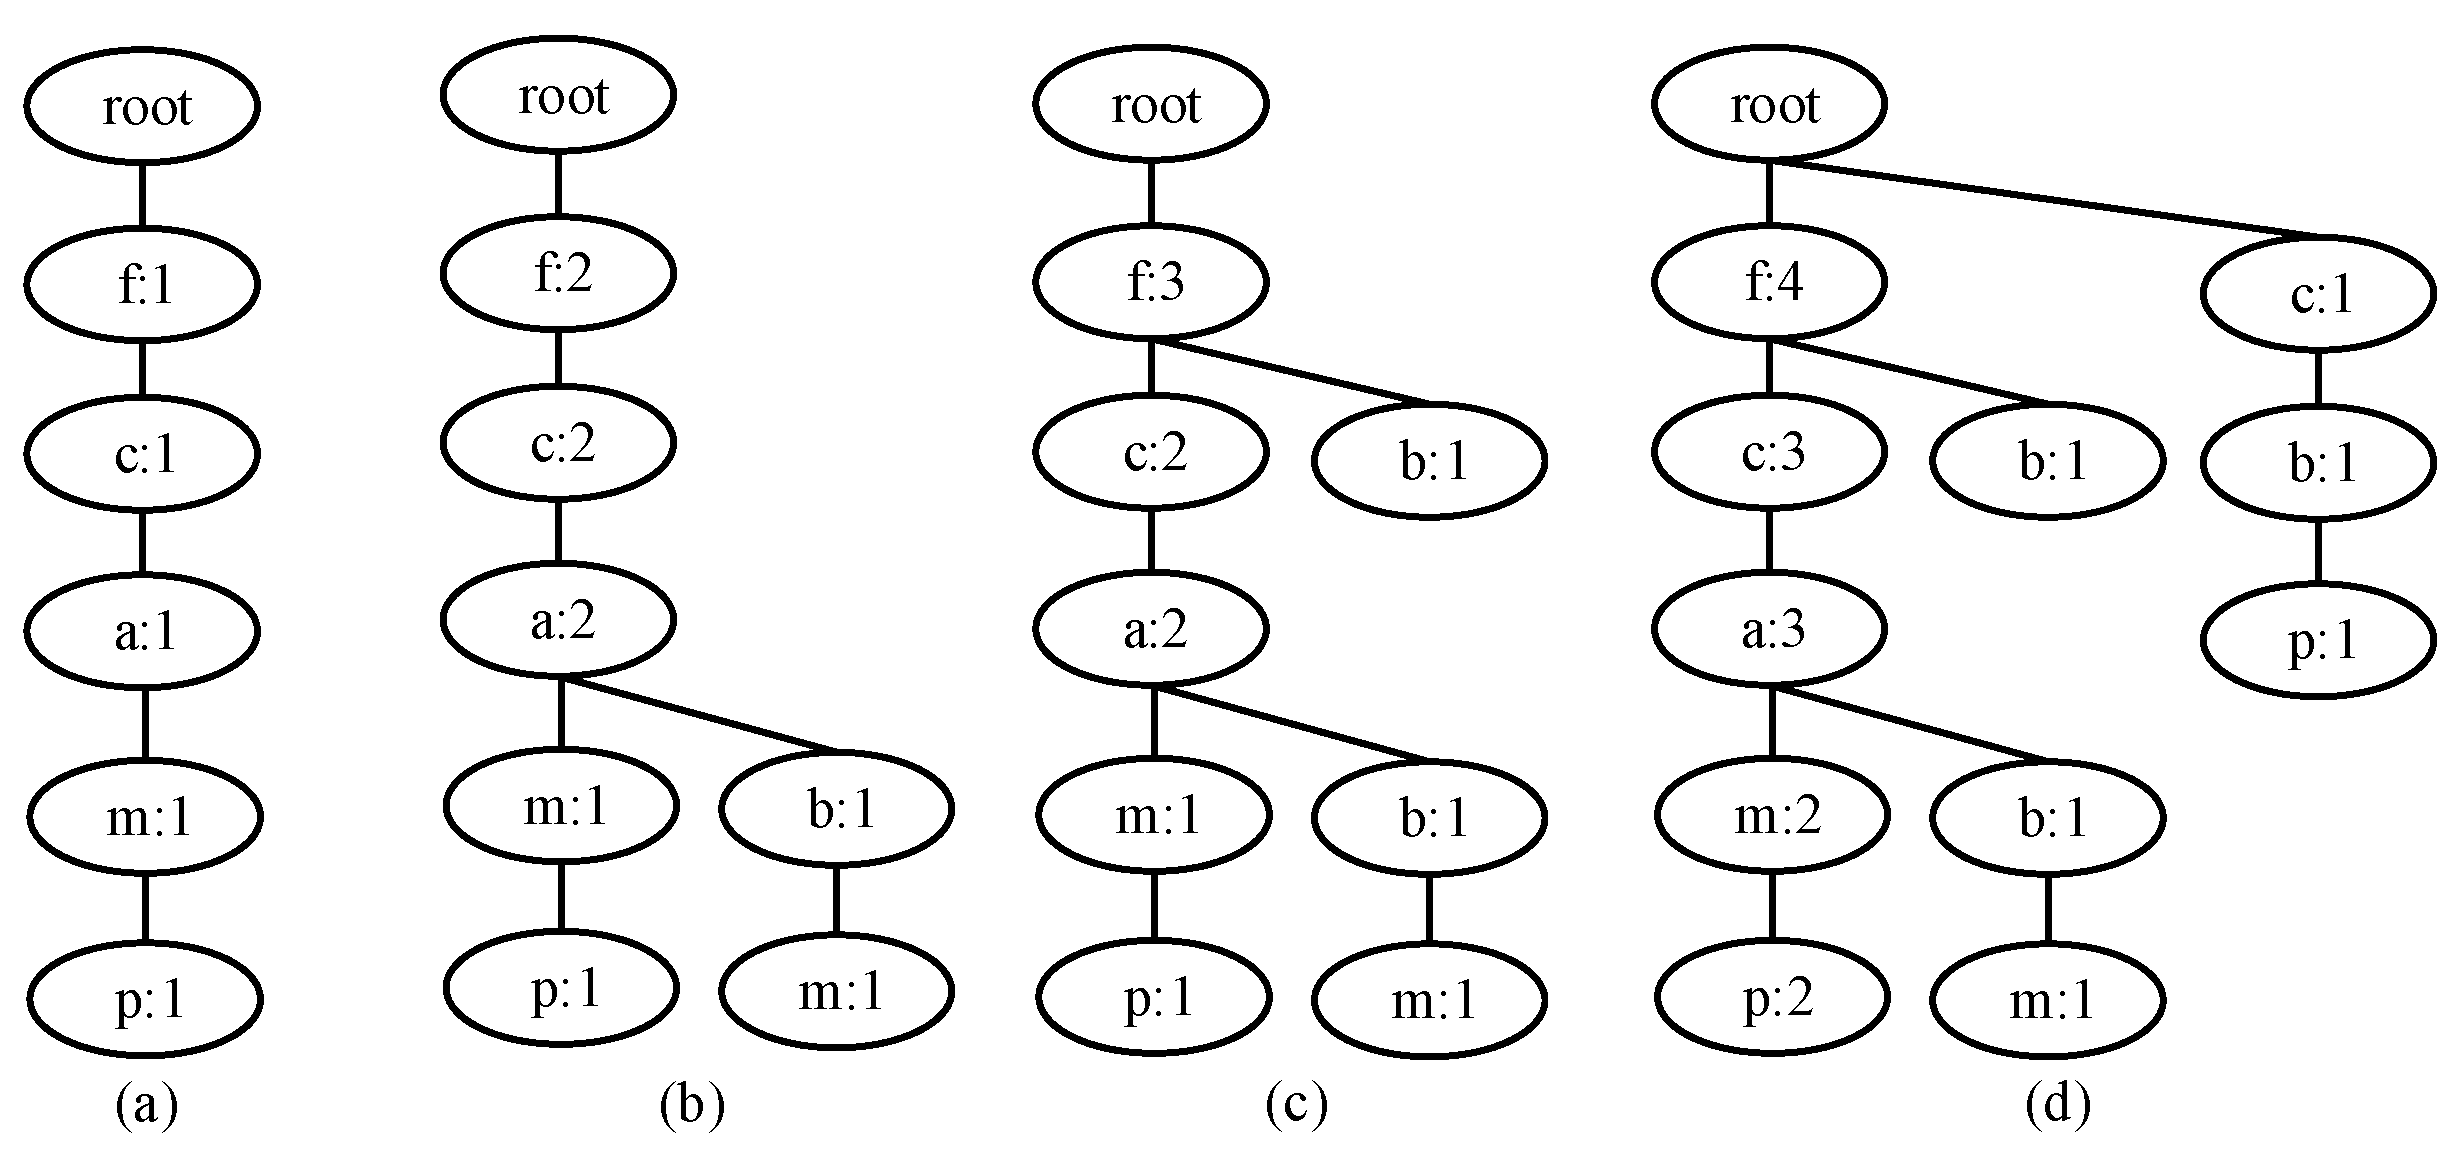
\includegraphics[width=0.6\textwidth]{img/FP-Growth.png}
    \caption{Process of FP-Tree construction. Adapted from \parencite{Jang2021FPGrowth}, based on \parencite{Han2000Mining}.}
    \label{fig:fp-growth}
\end{figure}

In addition to the tree structure, the FP-tree is accompanied by a frequent-item header table, which stores each item together with a pointer to the first node in the FP-tree containing that item. Each node in the tree is linked to the next node with the same item via a node-link, forming a linked structure across all occurrences of the same item~\parencite{Han2000Mining}.

The complete FP-tree:

\begin{figure}[H]
    \centering
    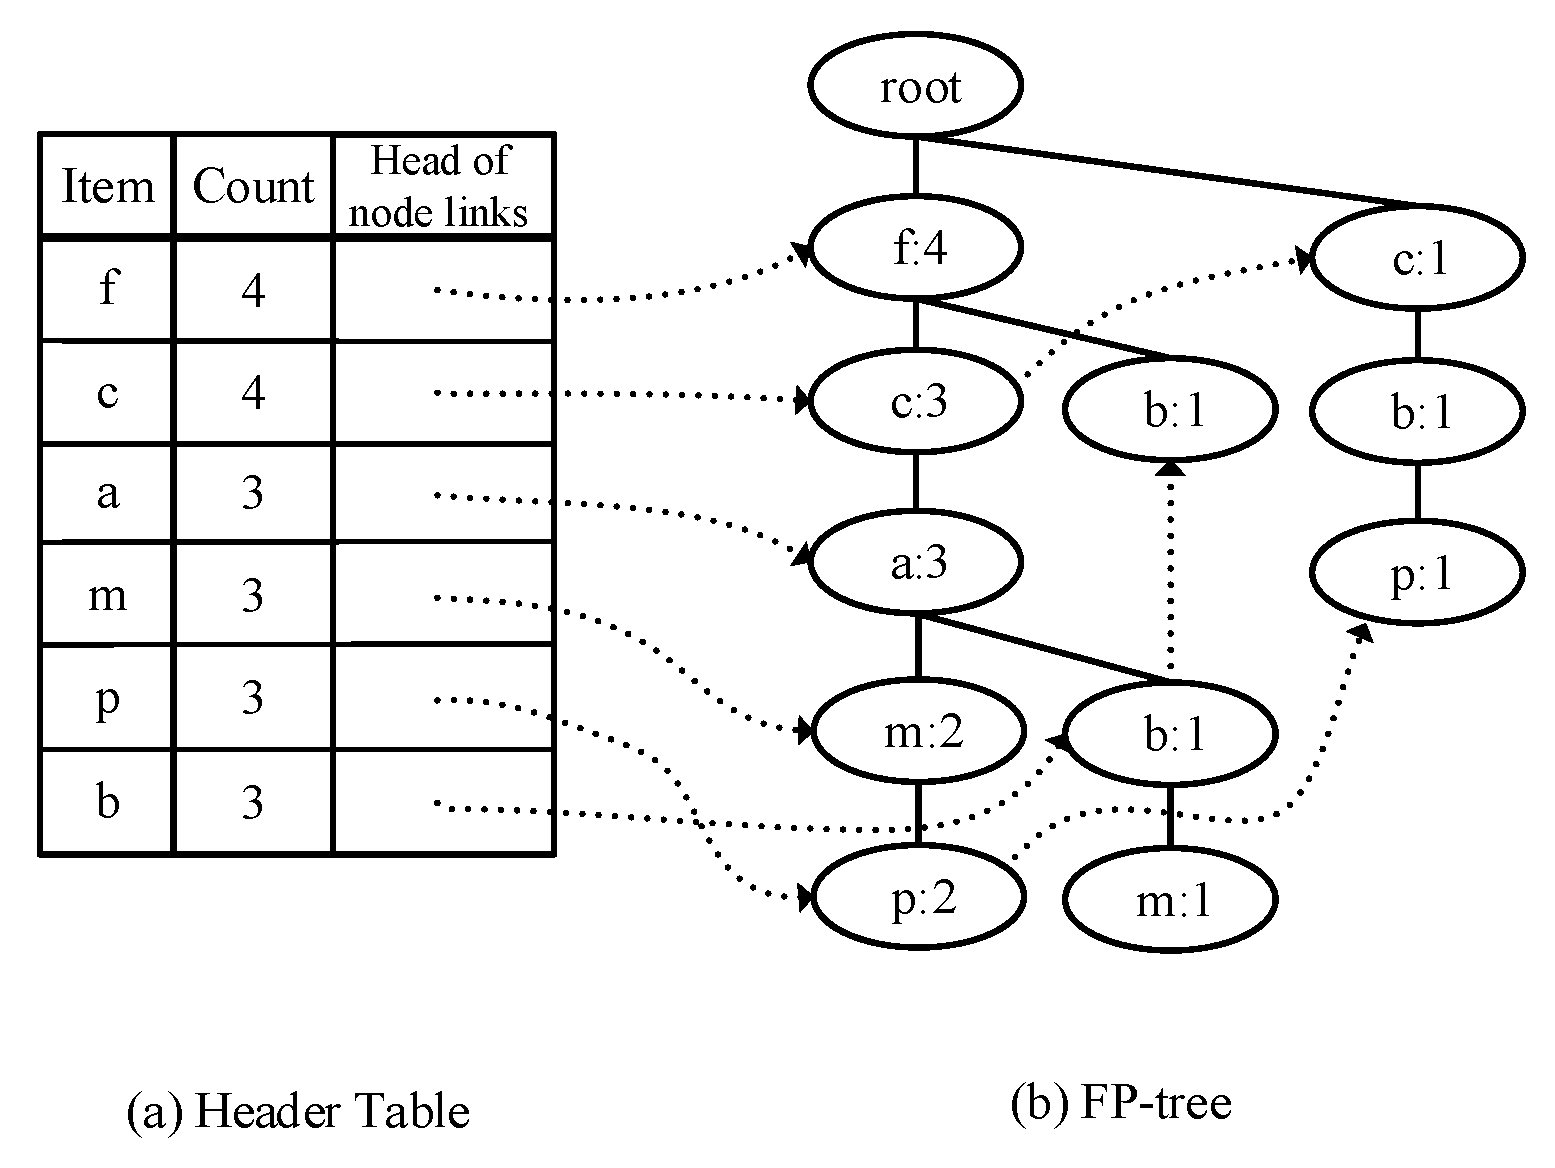
\includegraphics[width=0.6\textwidth]{img/FP-Growth2.png}
    \caption{Process of FP-Tree construction. Adapted from \parencite{Jang2021FPGrowth}, based on \parencite{Han2000Mining}.}
    \label{fig:fp-growth}
\end{figure}

Once the FP-tree has been built, the mining process proceeds by constructing the conditional pattern base for each frequent item. The conditional pattern base is the collection of prefix paths in the FP-tree that lead to a given item, excluding the item itself. Each path is annotated with its support count and represents the contexts in which the item occurs in the database~\parencite{Han2000Mining}.

A conditional FP-tree is constructed from the corresponding conditional pattern base. First, all infrequent items are removed from the prefix paths. In some cases, different prefix paths may become identical after pruning. For example, for item $m$ in Table~\ref{tab:conditional_fp_tree}, the prefix path ($f$:4, $c$:3, $a$:3, $b$:1, $m$:1) becomes ($f$:4, $c$:3, $a$:3, $m$:1) after removing item $b$. As a result, this path becomes identical to another path ($f$:4, $c$:3, $a$:3, $m$:2). Identical paths are merged, and their support values are added together. The prefix structure is preserved, while the support values of the paths are aggregated~\parencite{Han2000Mining}.

\begin{table}[h!]
\centering
\caption{Conditional pattern base and conditional FP-tree}
\label{tab:conditional_fp_tree}
\begin{tabular}{|c|p{8cm}|p{5cm}|}
\hline
\textbf{Item} & \textbf{Conditional Pattern Base} & \textbf{Conditional FP-tree} \\
\hline
$p$ & \{($f$:2, $c$:2, $a$:2, $m$:2), ($c$:1, $b$:1)\} & \{($c$:3)\}$\mid p$ \\
\hline
$m$ & \{($f$:4, $c$:3, $a$:3, $m$:2), ($f$:4, $c$:3, $a$:3, $b$:1, $m$:1)\} & \{($f$:3, $c$:3, $a$:3)\}$\mid m$ \\
\hline
$b$ & \{($f$:4, $c$:3, $a$:3, $b$:1), ($f$:4, $b$:1), ($c$:1, $b$:1)\} & $\emptyset$ \\
\hline
$a$ & \{($f$:3, $c$:3)\} & \{($f$:3, $c$:3)\}$\mid a$ \\
\hline
$c$ & \{($f$:3)\} & \{($f$:3)\}$\mid c$ \\
\hline
$f$ & $\emptyset$ & $\emptyset$ \\
\hline
\end{tabular}
\parbox{0.9\textwidth}{\centering \textit{Source: Han et al. (2000).}}
\end{table}

The final step of the FP-Growth algorithm is the generation of frequent itemsets from each conditional FP-tree. If the conditional FP-tree contains a single path, all combinations of items in the path are generated. Otherwise, frequent itemsets are mined recursively using conditional FP-trees~\parencite{Han2000Mining}.

\begin{table}[h!]
\centering
\caption{Frequent itemsets generated from conditional FP-trees}
\label{tab:frequent_itemsets}
\begin{tabular}{|c|p{10cm}|}
\hline
\textbf{Item} & \textbf{Frequent Itemsets} \\
\hline
$p$ & $\{\{p\}, \{c,p\}\}$ \\
\hline
$m$ & $\{\{m\}, \{f,m\}, \{c,m\}, \{a,m\}, \{f,c,m\}, \{c,a,m\}, \{f,c,a,m\}\}$ \\
\hline
$b$ & $\{\{b\}\}$ \\
\hline
$a$ & $\{\{a\}, \{f,a\}, \{c,a\}, \{f,c,a\}\}$ \\
\hline
$c$ & $\{\{c\}, \{f,c\}\}$ \\
\hline
$f$ & $\{\{f\}\}$ \\
\hline
\end{tabular}
\end{table}

Note that in Table~\ref{tab:conditional_fp_tree}, all conditional FP-trees correspond to single-path structures, which allows direct generation of all combinations of items within the path.

Consider a different example. Let the conditional pattern base of item $x$ be:
\{($a$:6, $b$:3), ($a$:6, $c$:3)\}. After aggregation, the conditional FP-tree consists of a single root node $a$ with two branches: $b$ and $c$, each with support 3.

Thus, the conditional FP-tree has a branching structure:
$a:6 \rightarrow \{b:3, c:3\}$.

In this case, frequent itemsets containing $x$ are generated recursively from the conditional FP-tree, resulting in:
\{$\{x\}$, $\{x,a\}$, $\{x,b\}$, $\{x,c\}$, $\{x,a,b\}$, $\{x,a,c\}$\}

However, the itemset \{$x,a,b,c$\} is not frequent, since there is no path in the conditional FP-tree that contains all three items simultaneously.

% \begin{table}[h!]
% \centering

% \begin{minipage}{0.23\textwidth}
% \centering
% \caption{Dataset}
% \label{tab:dataset_x}
% \begin{tabular}{|c|c|}
% \hline
% \textbf{TID} & \textbf{Items} \\
% \hline
% 100 & $\{x, a, b\}$ \\
% 200 & $\{x, a, b\}$ \\
% 300 & $\{x, a, b\}$ \\
% 400 & $\{x, a, c\}$ \\
% 500 & $\{x, a, c\}$ \\
% 600 & $\{x, a, c\}$ \\
% \hline
% \end{tabular}
% \end{minipage}
% \hfill
% \begin{minipage}{0.7\textwidth}
% \centering
% \caption{Conditional FP-tree construction (for item $x$)}
% \label{tab:cpb_x}
% \begin{tabular}{|c|p{6cm}|p{4cm}|}
% \hline
% \textbf{Item} & \textbf{Conditional Pattern Base} & \textbf{Conditional FP-tree} \\
% \hline
% $x$ & $\{(a,b):3,\ (a,c):3\}$ & $a:6 \rightarrow \{b:3, c:3\}$ \\
% \hline
% \end{tabular}
% \end{minipage}

% \end{table}

\subsection{Equivalence Class Transformation}

\subsection{Approximate / Probabilistic Frequent Itemset Mining}

\section{Association Rules}

\subsection{Definitions}

An association rule expresses the likelihood that the occurrence of one itemset increases the probability of another itemset. Formally, let $I$ be the set of all items and let $X$ and $Y$ be itemsets such that $X, Y \subseteq I$ and $X \cap Y = \emptyset$. An association rule is then defined as an expression $X \Rightarrow Y$~\parencite{agrawal1996fast}.

The confidence of this rule, sometimes referred to as accuracy, is defined as the support of the combined itemset $X \cup Y$ divided by the support of $X$ alone:
\[
\text{confidence}(X \Rightarrow Y, D) := P(Y \mid X) = \frac{\text{support}(X \cup Y, D)}{\text{support}(X, D)}
\]
~\parencite{Goethals2003}.

To further evaluate the strength of association between itemsets, an additional measure called Lift can be used. Lift is defined as the ratio between the joint probability of itemsets $X$ and $Y$ and the product of their marginal probabilities:
\[
\text{Lift}(X \Rightarrow Y) = \frac{P(X \cup Y)}{P(X)\,P(Y)}
\]
~\parencite{hussein2015using}.

The value of lift can be interpreted as follows: values greater than 1 indicate a positive correlation between itemsets $X$ and $Y$, meaning that the occurrence of $X$ increases the likelihood of $Y$. A value equal to 1 indicates statistical independence, while values less than 1 indicate a negative correlation, meaning that the occurrence of $X$ reduces the likelihood of $Y$~\parencite{Han2012}.

Support and confidence are among the most commonly used measures for discovering association rules. However, their main drawback is that they can be misleading, particularly in the case of frequently occurring items, which tend to achieve high support and confidence values. As a result, these measures do not necessarily reflect a true statistical dependency between items, but rather their high occurrence frequency in the dataset. For this reason, the lift measure can be used as a more reliable alternative for evaluating the strength of relationships between items. Lift compares the observed co-occurrence of items with the expected co-occurrence under the assumption of independence, and therefore better captures the actual statistical association between them~\parencite{hussein2015using}. 

\subsection{Example}

To illustrate the concept of association rules, consider the rule $c \Rightarrow a$ based on the dataset $D$ in Table~\ref{tab:dataset}.

\begin{table}[h!]
\centering
\caption{Transaction dataset}
\label{tab:dataset}
\begin{threeparttable}
\begin{tabular}{|c|c|}
\hline
\textbf{TID} & \textbf{Items} \\
\hline
1 & $\{a, b\}$ \\
2 & $\{a, c\}$ \\
3 & $\{a, b, c\}$ \\
4 & $\{a\}$ \\
5 & $\{b, c\}$ \\
6 & $\{a, c\}$ \\
7 & $\{b\}$ \\
8 & $\{a, b\}$ \\
\hline
\end{tabular}
\begingroup
\let\item\relax
\item \textit{Source: Author.}
\endgroup
\end{threeparttable}
\end{table}

The confidence of the rule $c \Rightarrow a$ is computed as:
\[
\text{support}(\{c, a\}, D) = 3
\]
\[
\text{support}(\{c\}, D) = 4
\]
\[
\text{confidence}(c \Rightarrow a, D) = \frac{3}{4} = 0.75
\]

The lift of the rule $c \Rightarrow a$ is computed as:
\[
P(c \cup a) = \frac{3}{8}, \quad P(c) = \frac{4}{8}, \quad P(a) = \frac{6}{8}
\]
\[
\text{Lift}(c \Rightarrow a) = \frac{3/8}{(4/8)(6/8)} = 1
\]

The confidence of the rule $c \Rightarrow a$ is 75\%. This suggests a relatively strong conditional association between $c$ and $a$. However, this interpretation can be misleading in terms of statistical dependence, since item $a$ is frequent in the dataset independently of $c$ and therefore occurs frequently regardless of the presence of $c$. In contrast, the lift value of 1 indicates statistical independence between $c$ and $a$, meaning that the occurrence of $c$ does not affect the probability of occurrence of $a$.

The goal of association rule mining is to discover frequent patterns in data rather than to directly perform predictive tasks such as classification~\parencite{Han2012}. Therefore, support and confidence are commonly used as the primary measures in association rule mining. However, association rules can also be adapted for predictive tasks through class association rules (CARs), in which the consequent is restricted to class labels, often achieving high predictive accuracy~\parencite{liu1998integrating}.

\subsection{Association Rule Mining}

\subsubsection{Definition}

Association rule mining (ARM) was first introduced by \textcite{Agrawal1993} and is commonly defined as a process of finding all association rules that satisfy a user-specified minimum confidence threshold. In the same work, a minimum support constraint is also introduced as a key practical requirement for efficient rule discovery.

In general, association rule mining can incorporate more types of constraints beyond support and confidence. These may include item-based (syntactic) constraints, length constraints limiting the size of rules, or other user-defined restrictions on the structure of discovered rules.

\subsubsection{Support Constraint}

Using only a minimum confidence constraint is not sufficient for practical association rule mining for several reasons.

First, confidence alone does not restrict the search space of itemsets, which results in an exponential number of candidate itemsets. In other words, all possible itemsets would need to be considered, which is computationally infeasible for large values of $m$, since the number of possible itemsets is $2^m$.

Second, confidence does not provide a measure of statistical significance. As a result, many rules may appear strong purely due to random chance in the data.

Finally, from a practical perspective, many of these rules are not useful for decision-making purposes~\parencite{Agrawal1993}.

\subsubsection{Process}

The ARM process is typically divided into two main steps. First, frequent itemsets are discovered from the transaction database. Second, association rules are generated from these frequent itemsets by evaluating whether they satisfy the minimum confidence constraint~\parencite{Agrawal1993}.

\subsubsection{Association Rules Generation}



\section{Action Rules}